\chapter{Technical and Theoretical Background}
\label{cap2a:background}
This chapter discusses the most important background concepts used in the current thesis. Namely, Section~\ref{sec:grippers_technolgy} is focused on explaining the existing gripper technologies and how devices and robots can grasp objects. Since a wide number of applications use multi-finger grasping, the theoretical background of this theme is presented in Section~\ref{sec:multifingered_grasping}. In the end, Section~\ref{sec:sim_ann} addresses the optimisation algorithm method embedded into the ``GraspIt!" simulator which is widely used by the academic community and further investigated in the current thesis proposal.  

%\clearpage
\section{Gripper Technologies}
\label{sec:grippers_technolgy}

End-effectors are hardware devices of handily mechanisms (e.g., robots and automation
systems) aiming them to interact with the environment.

Two classes of interaction are: passive and active.

In passive interaction, the end effectors are composed of sensors (e.g., inspection, quality assurance, and surveillance applications). Meanwhile, the active interaction consists of direct interaction with the workpiece (e.g., welding, cutting, drilling, screwing, grinding, painting, and grasping different objects).

\begin{figure}[h!]
\resizebox{0.85\textwidth}{!}{%
\begin{tcolorbox}
    \centering
    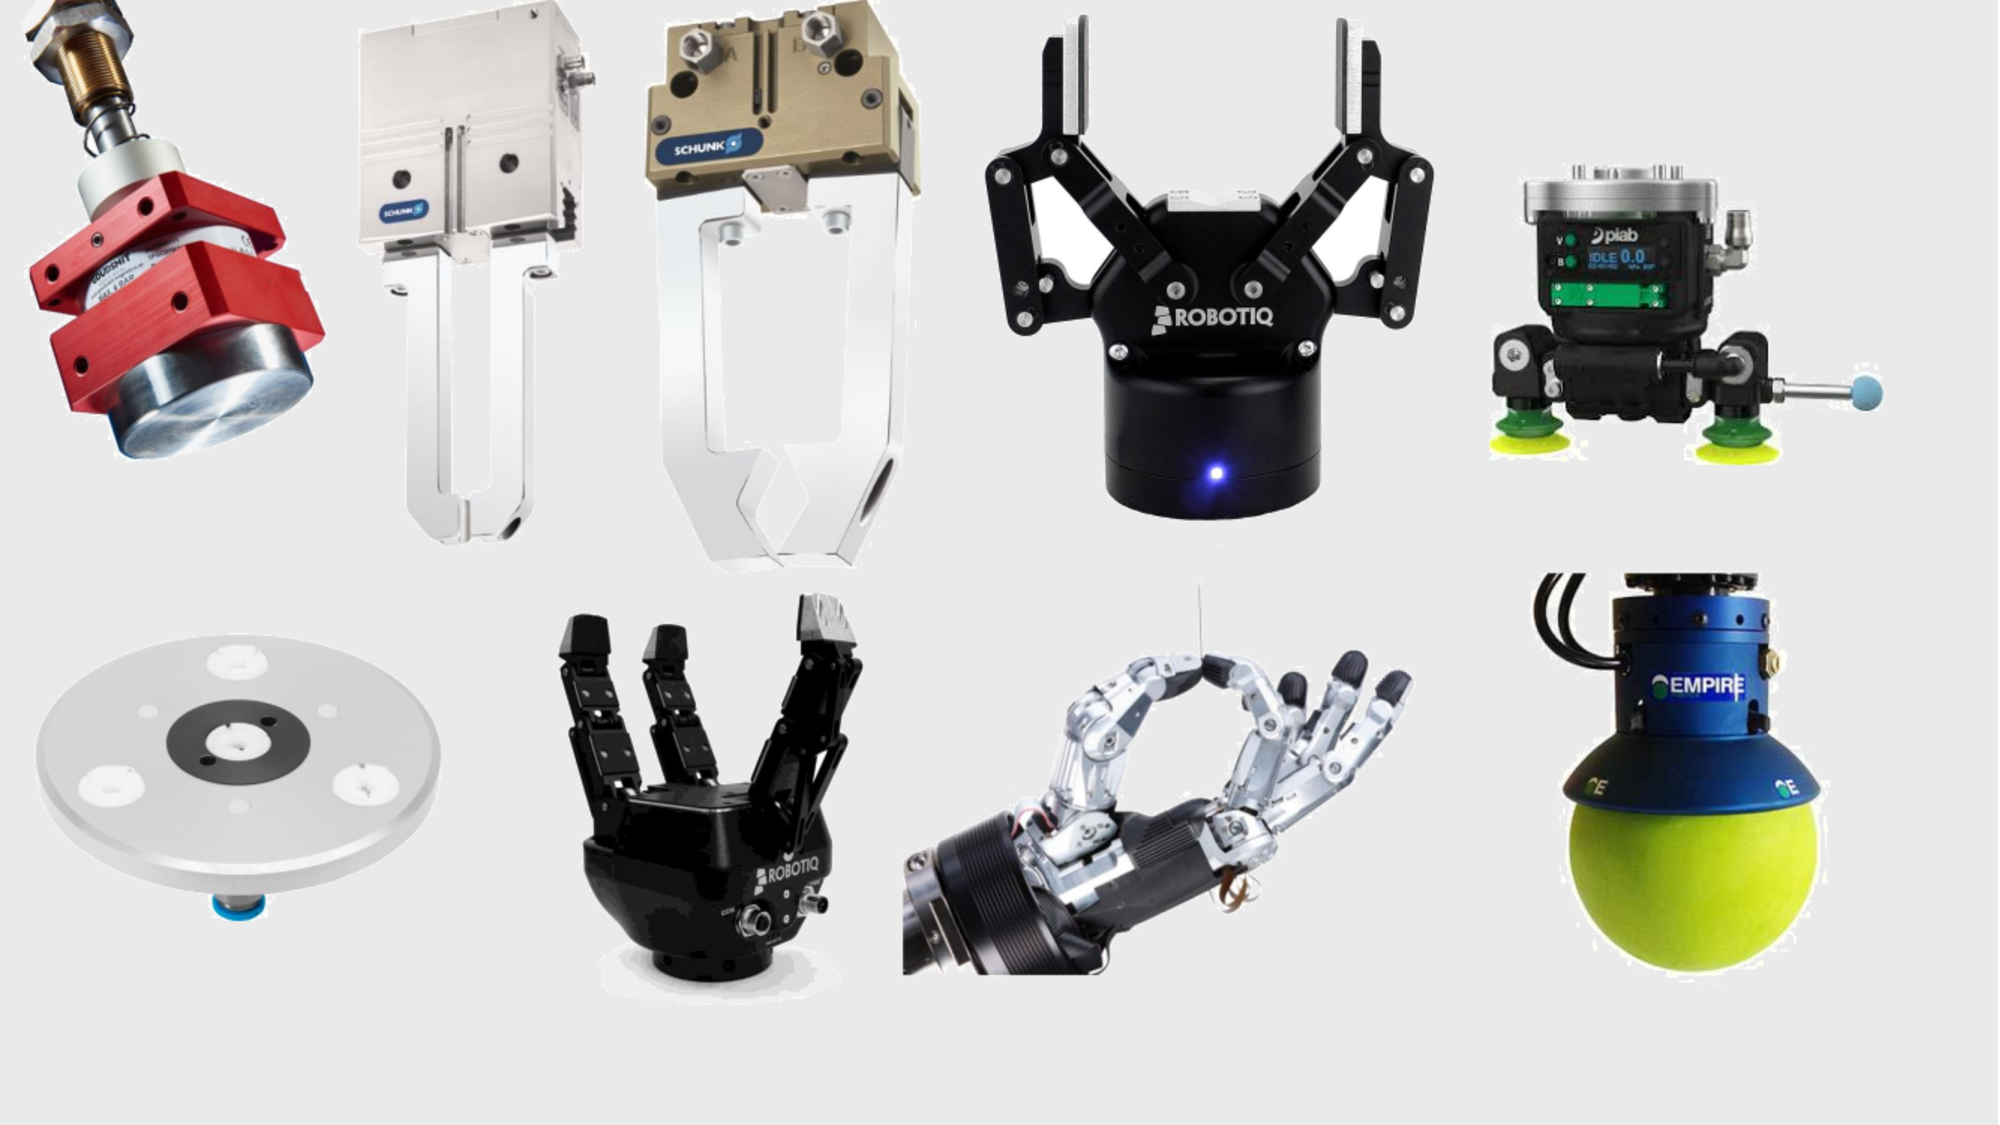
\includegraphics[trim={0mm 2cm 2cmm 0mm},clip,width=1\linewidth,angle=0]{Cap3/Figuras/grippers_list_gray_bg.pdf}
\end{tcolorbox}
    \caption{Commercial grippers examples. From top-left to down-right:  magnetic \cite{magnetic}, parallel fingers \cite{parallel}, angular fingers \cite{angular}, adaptive two-fingers \cite{robotiq_grippers}, dual suction \cite{dual_suction}, Bernoulli\cite{bernoulli}, adaptive three-fingers \cite{robotiq_grippers}, anthropomorphic \cite{anthopomorphic}, Versaball \cite{versaball}}
    \label{fig:gripper_examples}
    }%end of resize box
\end{figure}

The robotic grippers are a complex class of active end-effectors. They are active links to handle workpieces~\cite{monkman2007robot}. Grippers need to be flexible and versatile according to the application and object that they handle. Nowadays, with the development of new technologies, the variety of grippers and hardware allows more functionality, although it demands new efforts (e.g. modelling and control). In that way, hardware evaluation is also a part of the development of grasping estimation. The structure of the gripper defines a classification of grasping, related to the handling of the objects, i.e., hold an object with an emphasis in security (enveloping grasp) or dexterity and sensitivity (dexterous manipulation). The main characteristic of the dexterous is the manipulation of the object with fingers. Meanwhile, the enveloping grasping wraps the object with the palm and the finger \cite{Bicchi2000} and \cite{alonso2018current}.


Figure~\ref{fig:gripper_examples} and Figure~\ref{fig:most_usual_gripper_forms} elucidate some technologies applied in the concept of different
grippers. The most usual forms of grippers are \cite{monkman2007robot}:

\begin{itemize_jp}
    \item \textbf{Impactive}: the gripper realizes impactive forces against the surface of the workpiece. Some examples are the finger grippers.
    
    \item \textbf{Astrictive}: the gripper generates a field responsible for producing a binding force, as an air movement (vacuum suction), magnetic or electrostatic effect.
    
    \item \textbf{Contigutive}: the gripper touches a surface making contact prehension. The adhesion may be chemical or thermal effects.
    
    \item \textbf{Ingressive}: the gripper permeates the surface of the workpiece. This ingression can be intrusive (pins) or non-intrusive (e.g., hook and loop).    
\end{itemize_jp}

\begin{figure}[h!]
\resizebox{0.85\textwidth}{!}{%
\begin{tcolorbox}
     \centering
     \begin{subfigure}[c]{0.25\textwidth}
         \centering
         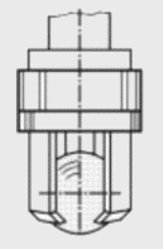
\includegraphics[width=.5\textwidth]{Apendices/Figuras/g1_gray_bg.pdf}
         \caption{Pure enclosing without clamping.}
         \label{fig:g1}
     \end{subfigure}
     \qquad
     \begin{subfigure}[c]{0.25\textwidth}
         \centering
         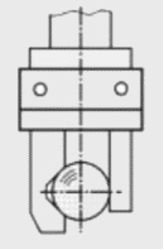
\includegraphics[width=.5\textwidth]{Apendices/Figuras/g2_gray_bg.pdf}
         \caption{Partial form fit combined with clamping force.}
         \label{fig:g2}
     \end{subfigure}
     \qquad
     \begin{subfigure}[c]{0.25\textwidth}
         \centering
         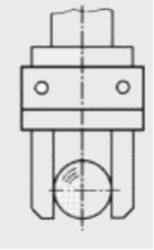
\includegraphics[width=.5\textwidth]{Apendices/Figuras/g3_gray_bg.pdf}
         \caption{Pure force closure.}
         \label{fig:g3}
     \end{subfigure}
	\qquad
     \begin{subfigure}[c]{0.25\textwidth}
         \centering
         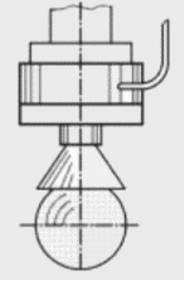
\includegraphics[width=.5\textwidth]{Apendices/Figuras/g4_gray_bg.pdf}
         \caption{Holding with vacuum air (pneumatic force closure).}
         \label{fig:g4}
     \end{subfigure}
     \qquad
     \begin{subfigure}[c]{0.25\textwidth}
         \centering
         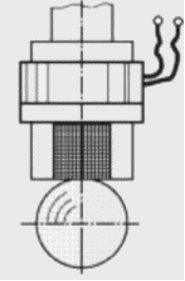
\includegraphics[width=.5\textwidth]{Apendices/Figuras/g5_gray_bg.pdf}
         \caption{Retention using magnetic field (force field).}
         \label{fig:g5}
     \end{subfigure}
     \qquad
     \begin{subfigure}[c]{0.25\textwidth}
         \centering
         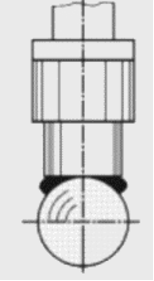
\includegraphics[width=.5\textwidth]{Apendices/Figuras/g6_gray_bg.pdf}
         \caption{Retention using adhesive media.}
         \label{fig:g6}
     \end{subfigure}
    \end{tcolorbox}
    \caption{Forms of grippers according to \cite{monkman2007robot}}
    \label{fig:most_usual_gripper_forms}
  }%end of resize box      
\end{figure}

The use of automatic tool change devices is an option to improve the flexibility, and
applicability of the grippers over the wide variety of objects and workpieces. Besides that, the use of handling machines or dual-arm robots in the automatic process is also a valid alternative (Figure~\ref{fig:alternatives}). Both solutions increase the complexity of the system, and the grasp estimation evaluation may determine which tool is best to complete the task to each object to grasp.

\begin{figure}[h!]
\resizebox{0.75\textwidth}{!}{%
\begin{tcolorbox}
    \centering
    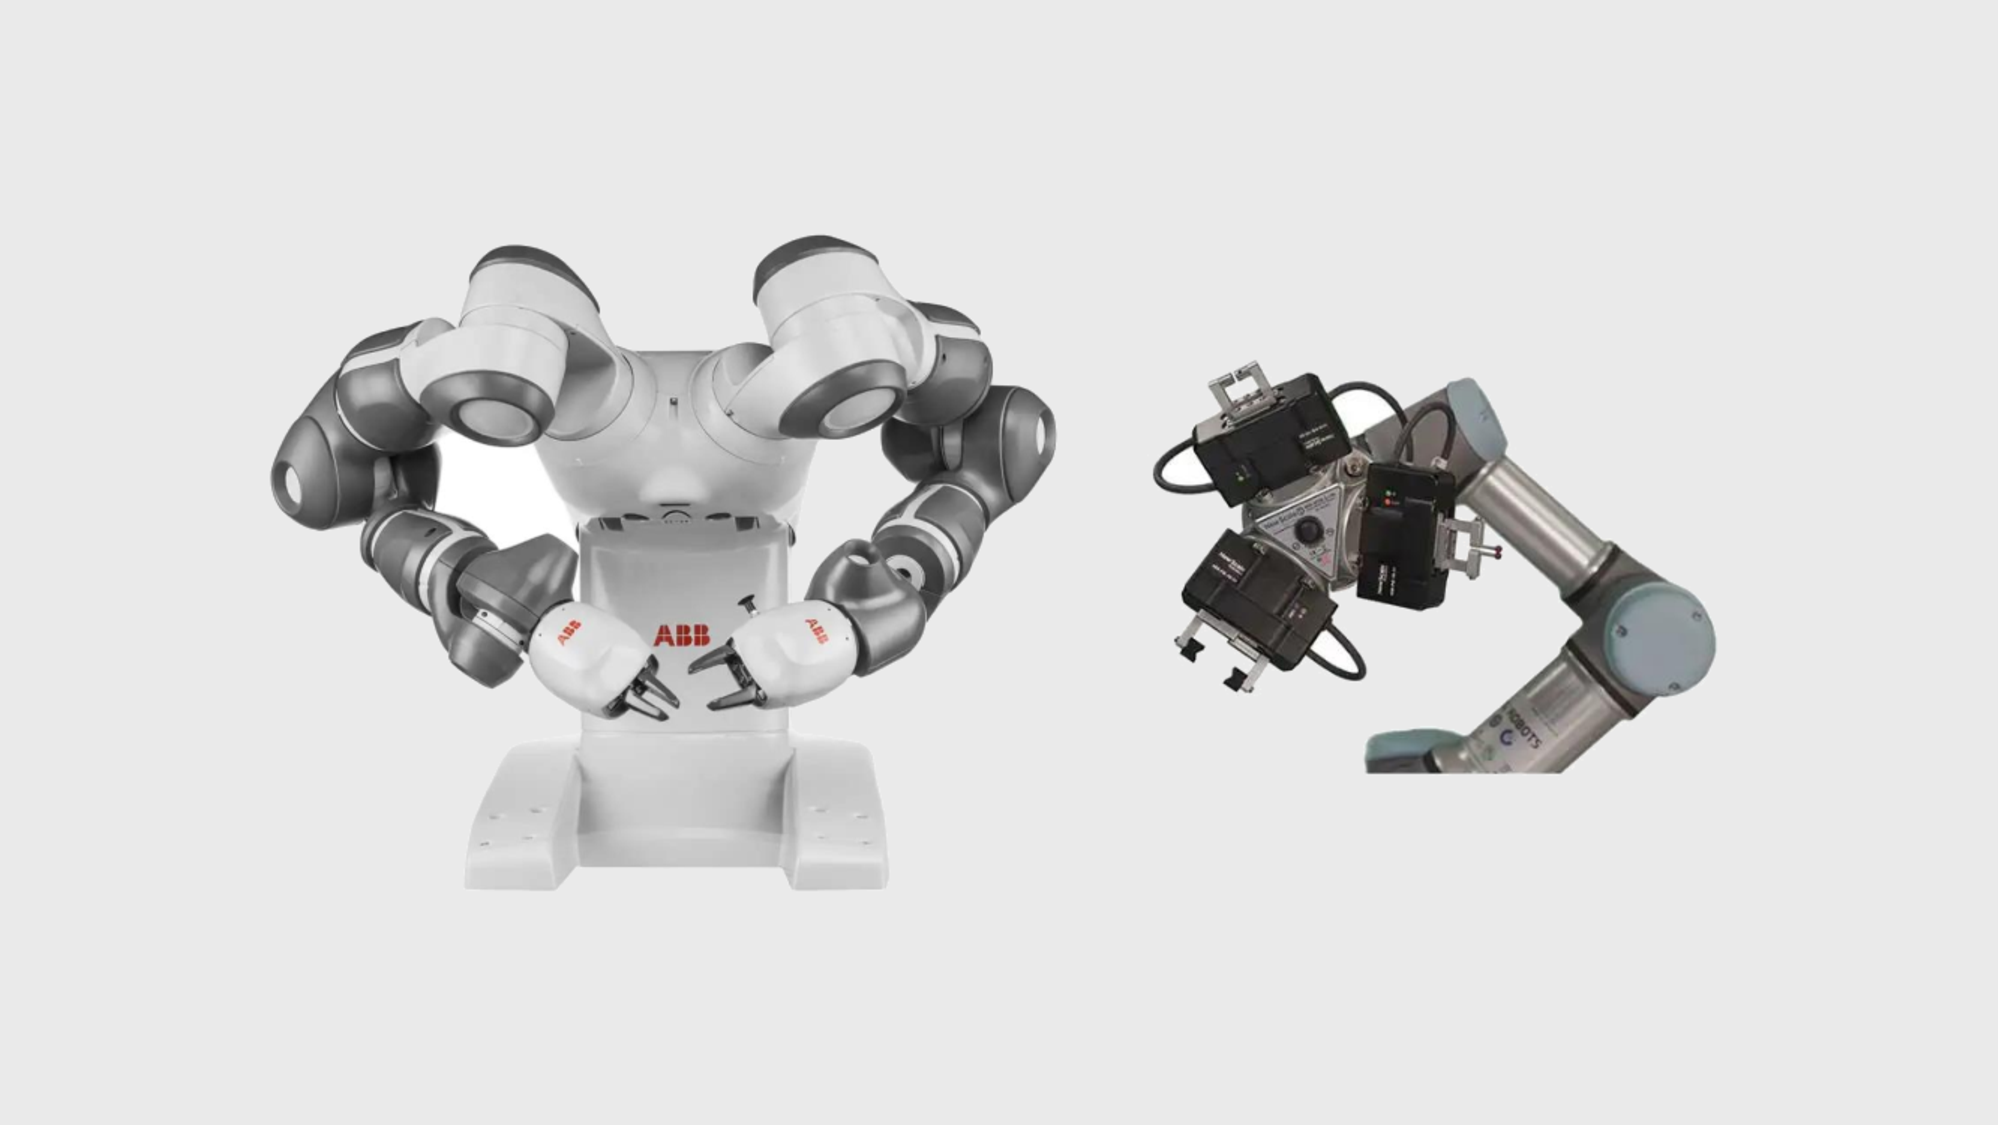
\includegraphics[trim={4cm 3cm 4cm 3cm},clip,width=1\linewidth,angle=0]{Apendices/Figuras/multi_end_effectors_gray_bg.pdf}
\end{tcolorbox}
    \caption{(left) Multi-arm robot~\cite{abb_dual_arm}. (right) Multi-gripper end-effector~\cite{multi_gripper_nsr}}
    \label{fig:alternatives}
}%end resize box
\end{figure}
%\clearpage
\section{Multi-Fingered Grasping}
\label{sec:multifingered_grasping}

A multi-fingered grasping is realised over a set of contacts between the active pairs (the workpiece and the gripper). Therefore, the determination of a suitable configuration of independent grasping points is the primary step of the fingered grasping planning. 

The wrench vectors describe the forces and moments that influence a rigid body's dynamic. These vectors can be used to formulate grasping locations, and a wrench vector is presented below:  

\begin{equation}
\mathbf{w_{c}}=\left[\begin{array}{l}
\mathbf{f} \\
\boldsymbol{\tau}
\end{array}\right]
\end{equation}

\noindent
where $\mathbf{f}$ and $\boldsymbol{\tau}$ are the vector representations of the forces and the moments. The wrench vectors have 3 and 6 \acp{DOF} in the case of $\mathbb{R}^2$ and $\mathbb{R}^3$, respectively.

The contact models can be categorised as friction-less contact, friction contact (also named hard finger contact), and soft contact~\cite{murray1994mathematical}. The focus of this chapter will be the friction contact, since this model covers the main application field of this thesis.

%The friction contact model considers the mechanical interaction between the active pairs. Therefore, the wrench convex depends on the friction contact forces, described by Coulomb model of friction: Considering the normal force $\mathbf{f_n}$, and the tangential force $\mathbf{f_t}$, static friction occurs when there is no slipping between the two surfaces of contact, that is when $\left|\mathbf{f_{t}}\right| \leq \mu_{t} |\mathbf{f_{n}}|
%$ where $\mu_{t} $ is a positive value representing the static tangential coefficient of friction. Figure~\ref{fig:friction_contact} shows an example of hard finger contact, the geometric representation of the Coulomb’s law and the friction cone convex also defined as ${FC}_{c_i}$. 

The friction contact model considers the mechanical interaction between the active pairs which is defined by Coulomb model of friction: Considering the normal force $\mathbf{f_n}$, and the tangential force $\mathbf{f_t}$, static friction occurs when there is no slipping between the two surfaces of contact, that is when $\left|\mathbf{f_{t}}\right| \leq \mu_{t} |\mathbf{f_{n}}|
$ where $\mu_{t} $ is a positive value representing the static tangential coefficient of friction. Figure~\ref{fig:friction_contact} shows an example of hard finger contact, the geometric representation of the Coulomb’s law and the friction cone convex also defined as ${FC}_{c_i}$. 

\begin{figure}[h!]
\resizebox{0.75\textwidth}{!}{%
\begin{tcolorbox}
\centerline{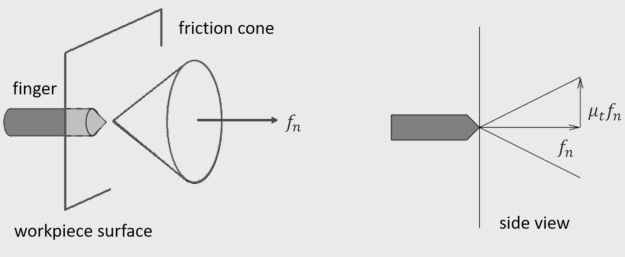
\includegraphics[trim={0cm 0cm 0cm 0cm},clip,width=1\linewidth,angle=0]{Apendices/Figuras/friction_contact_gray_bg2.pdf}}
\end{tcolorbox}
\caption{Friction contact model and the geometric representation of Coulomb’s law (figure based on~\cite{murray1994mathematical}).}
\label{fig:friction_contact}
} %end resize box
\end{figure}

A wrench representation, w.r.t the $i$-th contact point ($c_i$), could be defined as follows:

\begin{equation}
\mathbf{W_{c_i}}=\begin{bmatrix}
1 & 0 & 0 \\ 
0 & 1 & 0 \\ 
0 & 0 & 1 \\ 
0 & 0 & 0 \\ 
0 & 0 & 0 \\ 
0 & 0 & 0 
\end{bmatrix} \mathbf{f}_{c_i}, \quad \mathbf{f}_{c_i} \in F C_{c_i}
\end{equation}

\noindent
where $F C_{c_i}=\mathbf{f} \in \!R^3: \sqrt{f_{x}^{2}+f_{y}^{2}} \leq \mu_{t} f_{z,}, f_{z} \geq 0$, and $\mu_t$ is the transversal friction coefficient in $c_i$. 

Therefore, based on this wrench representation, it is possible to define the matrix that compose the wrench vector concept:

\begin{equation}
\mathbf{W}_{c_i}=\mathbf{B}_{c_i} \mathbf{f}_{c_i}, \quad \mathbf{f}_{c_i} \in F C_{c_i}
\end{equation}

\noindent
where $\mathbf{{B}_{c_i}}$ is the wrench basis matrix with dimension $p \times n$ where $p$ is the \acp{DOF} and $n$ the number of independent forces and moments that constitutes $\mathbf{{f}_{c_i}}$. The contact model discussed here has as reference frame the one with the origin coincident with the contact point itself. It is more convenient to refer all contacts in a grasp model to a common frame, generally the centre of mass of the work piece. Therefore the wrench transformation matrix is defined as follows:

\begin{equation}
^{o} \mathbf{Tw}_{c_i}=\left[\begin{array}{cc}
{^{o} \mathbf{R}_{\mathrm{c_i}}} & {0} \\
{^o \hat{\mathbf{t}}_{\mathrm{c_i}} {}^{o} \mathbf{R}_{\mathrm{c_i}}} & {^{o} \mathbf{R}_{\mathrm{c_i}}}
\end{array}\right]
\in \mathbb{R}^3
\end{equation}

\noindent
where $ ^o\mathbf{R}_{c_i}$ and $^o\mathbf{t}_{c_i}$ are the rotation and translation matrix of the $i$-th contact point ($c_i$) w.r.t. object frame ($o$). The $\mathbf{\hat{t}}$ is the linear operator representing the cross product $^o\mathbf{t}_{c_i} \times {{{}^o}\mathbf{R}}_{c_i}$ as bellow:

\begin{equation}
\widehat{\boldsymbol{a}}=\left[\begin{array}{ccc}
0 & -a_{3} & a_{2} \\
a_{3} & 0 & -a_{1} \\
-a_{2} & a_{1} & 0
\end{array}\right] \quad where \quad \boldsymbol{a} = \left[\begin{array}{c}
a_{1} \\
a_{2} \\
a_{3}
\end{array}\right]
\end{equation}


Hence, the contact map $\mathbf{G}_{i}$ is defined as follows:

\begin{equation}
\mathbf{G}_{i}=^{o} \mathbf{T} \mathbf{w}_{c_i}^{\prime} \mathbf{B}_{c_i}
\end{equation}

Note that it describes the direction of each component of the $i$-th applied wrench and defines the constraints of the contact. The grasp map is the matrix with all contact maps that characterise the contact model (it is also named constraint matrix):

\begin{equation}
\mathbf{G}=\left[\begin{array}{llll}
{{}^o \mathbf{T} \mathbf{w}_{c_1}^{\prime} \mathbf{B}_{c_1}} & {\dots} & {{}^{o} \mathbf{T} \mathbf{w}_{c_N}^{\prime} \mathbf{B}_{c_N}}
\end{array}\right]
\end{equation}

Then, including the magnitude of the forces, a workpiece wrench can be written:

\begin{equation}
^{o} \mathbf{W}=\left[\mathbf{G}_{1}, \ldots, \mathbf{G}_{N}\right]\left[\mathbf{f}_{c_1}, \ldots, \mathbf{f}_{c_N}\right]^{\prime}=\mathbf{G} \mathbf{F}
\end{equation}

\noindent
where: $\mathbf{F} \in F C \text { and } F C=F C_{c_1} \times \ldots \times F C_{C_N}$

The grasp map is an important matrix since it is the mathematical formulation of a multi-finger grasping. From now on, the common reference frame is defined as the object frame, and for convenience, the $^{o}\mathbf{W}$ will be substituted by $\mathbf{W}$. Each column of $\mathbf{W}$ represents the independent contact wrenches. All the contacts discussed here are punctual contacts since the other kinds of contact can be approximate by a set of punctual contacts and edge contacts.

By means of the convex linearisation of the friction contact, Figure~\ref{fig:friction_contact_linearised}, it is possible to represent the contact force ($\mathbf{f}_{c_i}$) as a linear combination of the cone edges ($\mathbf{S}_{c_i}$) and ($a_d$):

\begin{figure}[h!]
	\resizebox{0.75\textwidth}{!}{%
		\begin{tcolorbox}
			\centerline{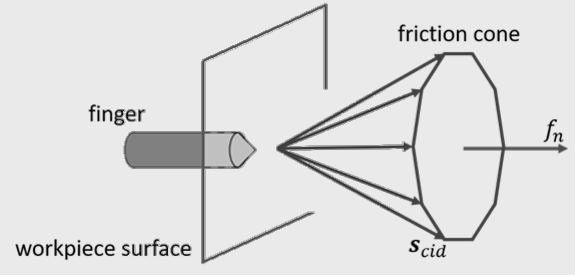
\includegraphics[trim={0cm 0cm 0cm 0cm},clip,width=1\linewidth,angle=0]{Apendices/Figuras/friction_contact_linearised.pdf}}
		\end{tcolorbox}
		\caption{Linearised friction contact model.}
		\label{fig:friction_contact_linearised}
	} %end resize box
\end{figure}


\begin{equation}
	\mathbf{f}_{ci} \approx \sum_{d=0}^{D} a_{d} \mathbf{s}_{ci_d}, a_{d} \geq 0 \quad, \quad \sum_{d=0}^{D} a_{d}=1
\end{equation}

where D is the number of edges that composes the linearised cone. A matrix notation can be formed as:

\begin{equation}
	\mathbf{f}_{ci}=\mathbf{A} \mathbf{S}_{ci}^{\prime}
\end{equation}

with $\mathbf{A}=\left[a_{0}, \ldots, a_{D}\right]$ and $\mathbf{S}_{ci}=\left[\mathbf{s}_{ci_0}, \ldots, \mathbf{s}_{ci_D}\right]$

Therefore, including all contact forces, the $\mathbf{W}$ associate with $\mathbf{S}$ is called primitive grasp map, also referred as primitive wrench map, defined as follow:

\begin{equation}
	\mathbf{W}_{p}=\left[\mathbf{G}_{1}, \ldots, \mathbf{G}_{N}\right]\left[\mathbf{A} \mathbf{S}_{c 1}^{\prime}, \ldots, \mathbf{A} \mathbf{S}_{c N}^{\prime}\right]^{\prime}=\mathbf{G} \mathbf{F}_{\mathbf{p}}
\end{equation}

The columns of $\mathbf{W}_{p}$ represent all wrenches associated with the edges of the linearised friction cone of the N contacts. It is an interesting matrix since it defines boundary conditions of contact. Applying a torque factor $\alpha$ (ensuring $|\tau| \leq|F|$) in each $w_{pd_{ci}}$ in $\mathbf{W}_{p}$, i.e.:

\begin{equation}
	w_{c}=\left[\begin{array}{c}
		\boldsymbol{f} \\
		\alpha \boldsymbol{\tau}
	\end{array}\right]
\end{equation}

and defining $\alpha=\frac{1}{r}$, where $r$ is the maximum radius of the centre of mass or gravity of the object and a contact point, it is possible to evaluate the grasps independently of the object size.

The $\mathbf{W}_p$ of all contact forces also defines the GWS (grasp wrench space) of the grasping. It is obtained by means of the $L_\infty$ or $L_1$ norm over the vector $\mathbf{g}$ composed by the magnitude of each contact normal force. The $L_\infty$ defines the GWS($W_L\infty$) considering the limitation of the maximum allowable normal contact force, while $L_1$ defines the GWS($W_{L1}$) by the sum magnitude of the normal contact forces. The norms operation yields to:


\begin{equation}
\begin{aligned}
\mathbf{W}_{L_{1}} &=\text { ConvexHull }\left(\bigcup_{c_i}^{N} \mathbf{w}_{p_1 c_i}, \ldots, \mathbf{w}_{p D_{c_i}}\right) \\
\mathbf{W}_{L_{\infty}} &=\text { ConvexHull }\left(\bigoplus_{c i}\left\{\mathbf{w}_{p_1 c_i}, \ldots, \mathbf{w}_{p D_{c_i}}\right\}\right)
\end{aligned}
\end{equation}

\noindent
where $\mathbf{w}_{pd_{ci}}$ $\in$ $\mathbf{W}$ and $\bigoplus$ is the Minkowski sum. More detail about the norm operation can be verified in~\cite{Ferrari}.


The concept of grasp closure evaluates the restraining of an object. A common assumption is the force-closure implies an equilibrium, but the inverse does not apply. A grasp has its convex hull defined by the wrenches that constitute the grasp configuration, i.e., the matrix $\mathbf{W}$. In a force-closure grasp, the convex hull includes the wrench space origin $\{O\}$, see Figure~\ref{fig:gws_force_closure}. According to the definition presented in~\cite{salisbury1983kinematic}, if all wrenches in $\mathbf{W}$ positively span the entire wrench space, the grasp will be force-closure. Figure~\ref{fig:gws_force_closure} shows a  grasp wrench space (GWS) and a convex hull of grasp configuration for force and non-force-closure, for a planar case with a fixed value for the moment ($\tau$) in the z-axis. Therefore, it is considered $\mathbf{f}_{c_i} \in  \mathbb{R}^2:  {f}_{c_i}  = (f_{x} , f_{y})$, and  the resistance to perturbation in both force axes is evaluated. 

\begin{figure}[h!]
\resizebox{0.8\textwidth}{!}{%
\begin{tcolorbox}
\centerline{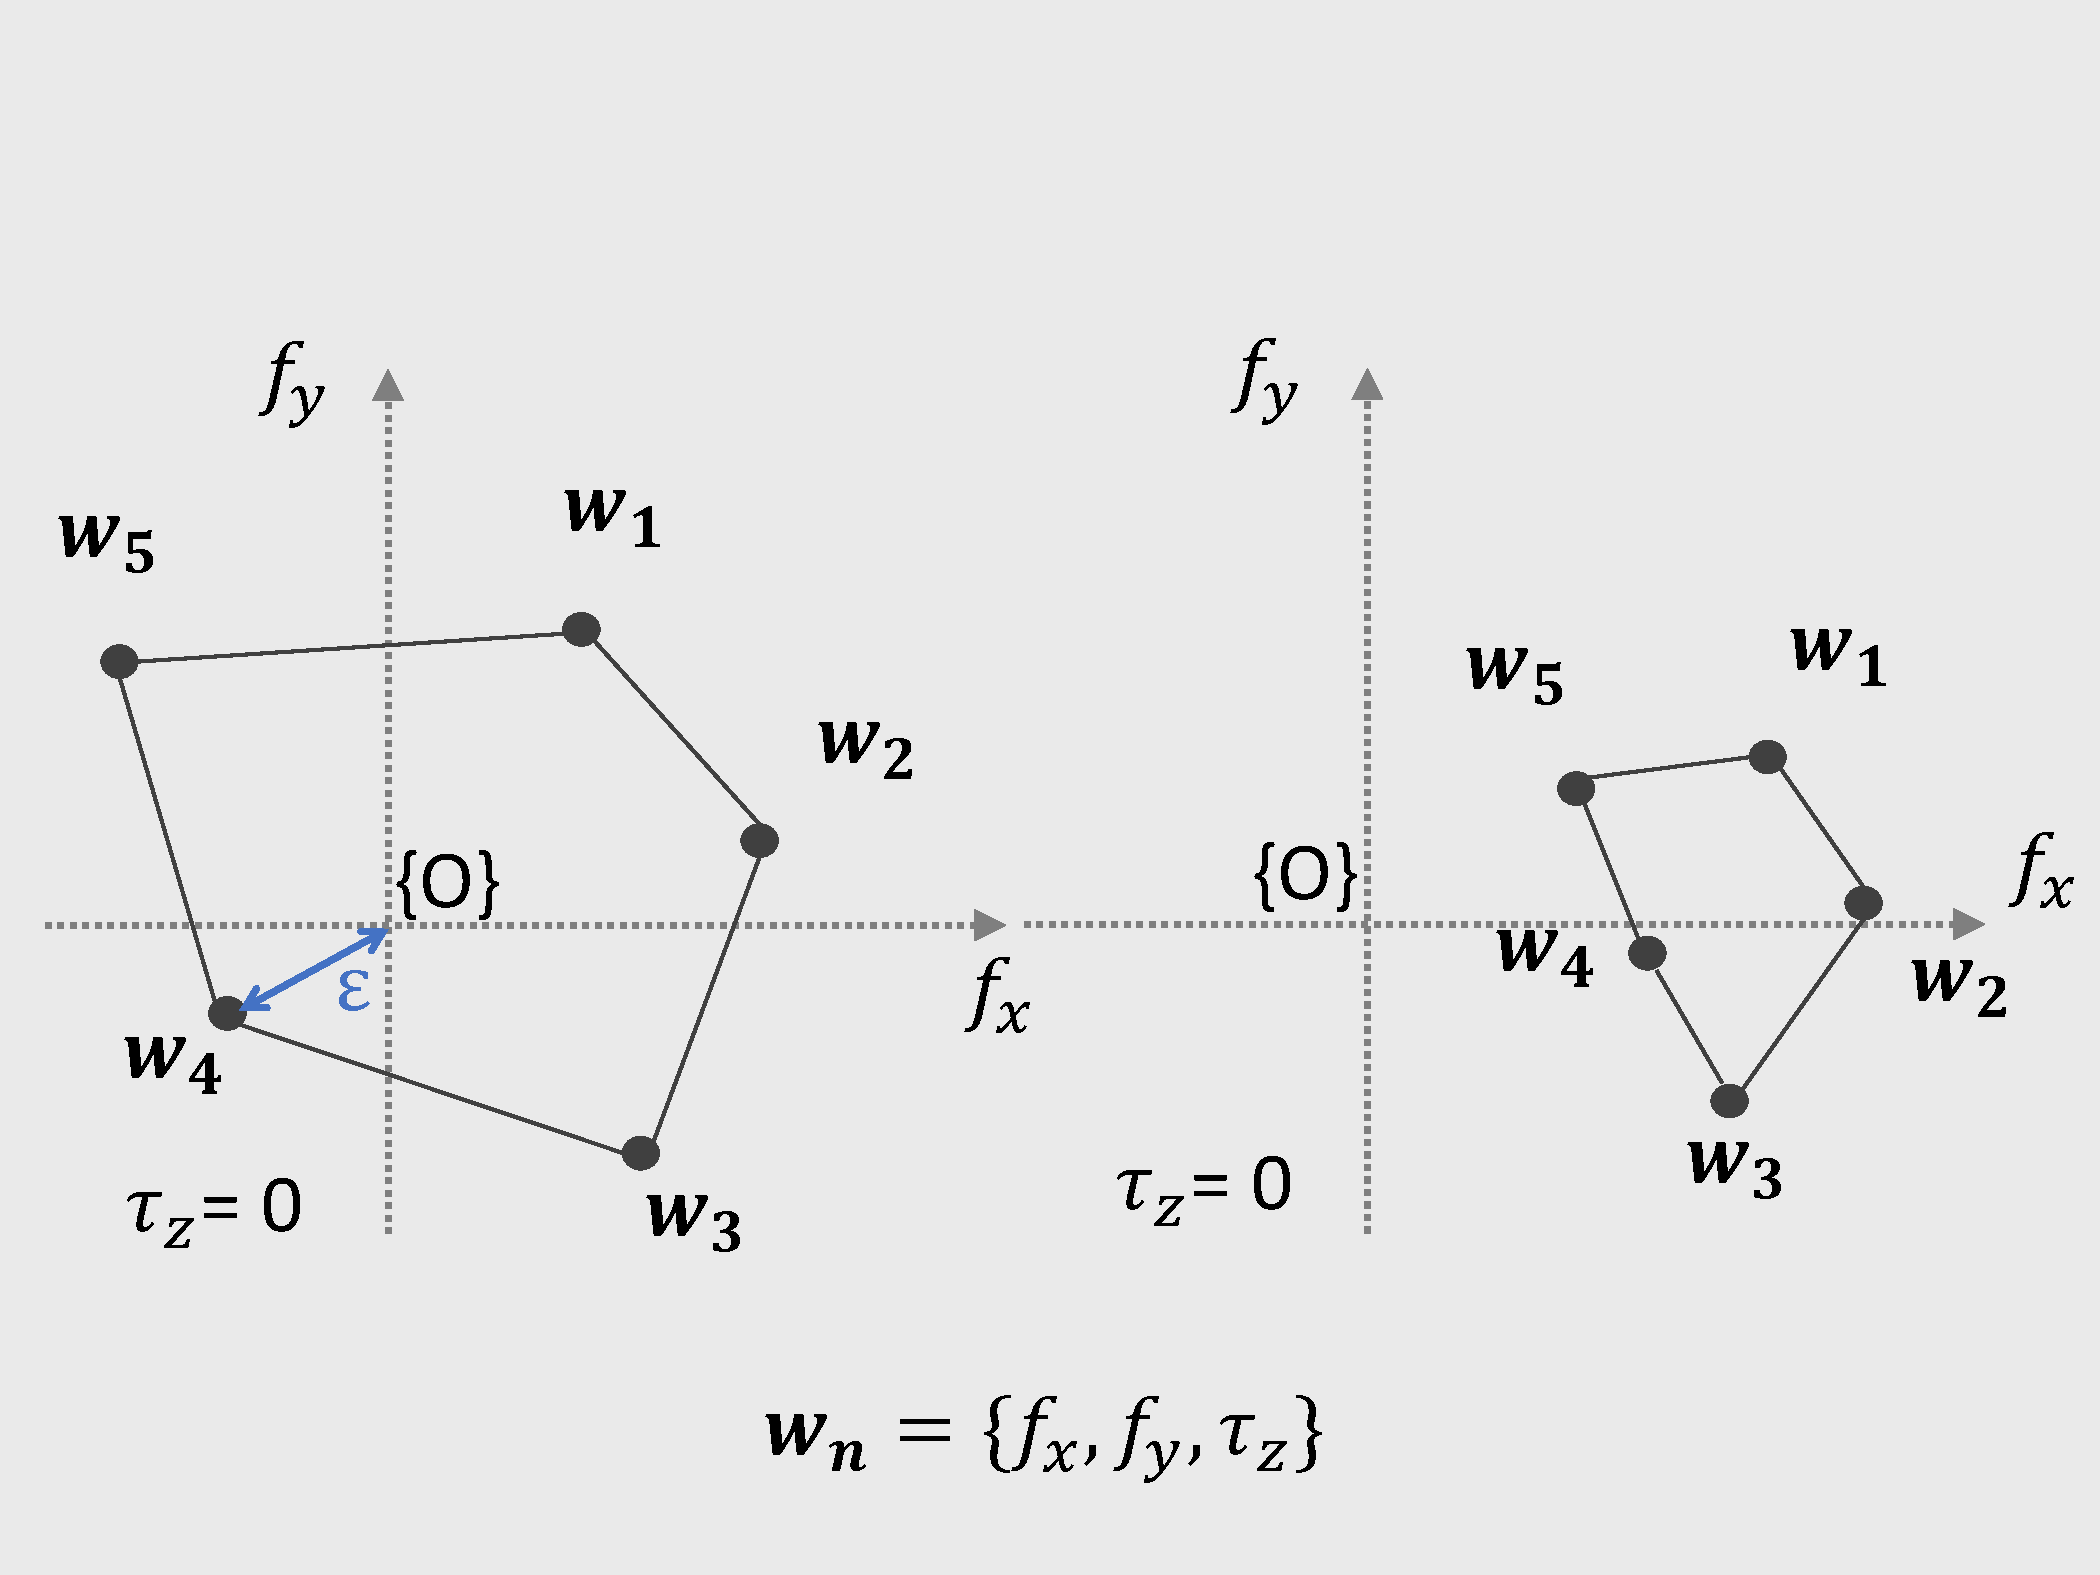
\includegraphics[trim={0cm 1.2cm 0cm 5.5cm},clip,width=1\linewidth,angle=0]{Cap2/Figuras/wrenchspace_anlayses_2.pdf}}
\end{tcolorbox}
\caption{Wrench convex-hull configuration. Force-closure and the $\epsilon$-value (left). Non-force-closure (right).}
\label{fig:gws_force_closure}
}%end resize box
\end{figure}

Since several configurations can reach a force-closure grasp, quality metrics like $\epsilon$-metric evaluate which one is best. The $\epsilon$ is a normalized value that represents the wrench vector's distance to the origin ($\{O\}$), which is the shortest, i.e., the worst wrench vector to support an external perturbation. An efficient grasp, ideally, has $\epsilon=1$ . The left GWS of Figure~\ref{fig:gws_force_closure} elucidates this metric and the readers are encouraged to a more detailed review of this grasping definition in~\cite{Ferrari}.



%\clearpage
\section{Simulated Annealing Grasping}
\label{sec:sim_ann}

The \ac{SANN} algorithm~\cite{Ciocarlie2009} integrated in the ``GraspIt!'' simulator~\cite{AndrewT2004} is one of the tools that the grasping pipeline relies on. Since it was used from the perspective of an end user, a brief explanation will be done here, and any further information can be retrieved on the referenced papers.

The \ac{SANN} is a heuristic optimization algorithm based on the cooling of a set of atoms to a minimum state of energy, and it was first introduced by~\cite{kirkpatrick1983} in a Statistical Mechanics optimization algorithm application. The ``Very Fast Simulated Re-Annealing'' was an improvement made by Ingber at~\cite{ingber1988} and used here. Since it is based on temperature, Ingber proposed that its cooling process decrease as described by Equation~\ref{eq:temperature}

\begin{equation}
T=T_{0} \cdot exp{(-k^{1/D})}
\label{eq:temperature}
\end{equation}

\noindent
where $D$ is the dimensional search space, $k$ a \ac{SANN} parameter step, and $T_0$ is the initial temperature.

Each algorithm iteration generates new state variables following a rule of neighbouring. Considering current and a new variable state as $S_{current}$ and $S_{new}$, this rule yields Equation~\ref{eq:neighbors}.

\begin{equation}
S_{new}=S_{current}+T \cdot(-1)^{round(Rand(0,1))} \cdot\left(1+\frac{1}{T}\right)^{Rand(-1,1)}
\label{eq:neighbors}
\end{equation}

\noindent
and the probability to change the state between the current and the new one is defined by Equation~\ref{eq:very_fast_snn_prob} where $Q(\bullet)$ represents the objective function of the optimization problem.

\begin{equation}
exp({\frac{Q(S_{current})-Q(S_{new})}{T}})>Rand(0,1)
\label{eq:very_fast_snn_prob}
\end{equation}

Regarding the multi-fingered grasping, it is possible to define a state based on the hand posture $\mathbf{p}$ and, the position and orientation of the wrist $\mathbf{w}$ such as:

%\begin{equation}
%S=[\mathbf{p}, \mathbf{w}], \quad \mathbf{p} \in \mathcal{R}^{d}, \mathbf{w} \in \mathcal{R}^{6}
%\label{eq:fob_grasp}
%\end{equation}

\begin{equation}
	\mathbf{S}=\left[\begin{array}{c}
		\mathbf{p} \\
		\mathbf{w}\end{array}\right], \quad \mathbf{p} \in \mathcal{R}^{d}, \mathbf{w} \in \mathcal{R}^{6}
\label{eq:fob_grasp}
\end{equation}

\noindent
where $d$ is the number of intrinsic \acp{DOF} of the hand. For instance, the human hand and the robotic Barrett gripper~\cite{barret_hand} have 20 \acp{DOF} and 4 \acp{DOF}, respectively.

As discussed by~\cite{Ciocarlie2009}, the hand posture is defined by \textit{eigengrasps}, a subspace of movement based on how human generate hand postures. The \textit{eigengrasps} reduces the \acp{DOF} of the hand based on how humans select appropriate grasps and hand postures in a primitive fashion. Studies show that humans simplify, unconsciously, the problem with a pattern in the movement. More information can be verified in~\cite{Ciocarlie2009,Santello2002}. 

Considering a hand with $d$ hand's postures DOFs, it is possible to defined a d-dimensional \textit{eigengrasp} ($\mathbf{e}_i$) as:

\begin{equation}
	\mathbf{e}_{i}=\left[\begin{array}{llll}
		e_{i, 1} & e_{i, 2} & \ldots & e_{i, d}
	\end{array}\right]
\end{equation}

\noindent where each $e_{i,d}$ represents the individual joint direction movement. In other words, the \textit{eigengrasp} ($\mathbf{e}_i$) is a d-dimensional direction vector that represents the motion of a group joint space. Therefore, it is possible to create a set of \textit{eigengrasps} with size $b \ll  d$, simplifying the searching space. Hence, a posture can be defined by Equation~\ref{eq:eigengrasp_posture}.

\begin{equation}
p=\mathbf{p}_m+\sum_{i=1}^{b} a_{i} \mathbf{e}_i
\label{eq:eigengrasp_posture}
\end{equation}


\noindent
with posture origin defined by $\mathbf{p}_m$ and $b$ the total number of \textit{eigengrasps}. Since it is a linear combination, the parameter array $\mathbf{a} = [a_1, a_2, ... , a_b]$  will be the optimisation variable in Equation~\ref{eq:fob_grasp} together with the $\mathbf{w}$. Therefore, the dimensional search space $D$ has a reduced length, i.e. $D = sizeof(\mathbf{a}) +  sizeof(\mathbf{w})$. The Figure~\ref{fig:barrett_eigengrasps} elucidates the \textit{eigengrasp} discussion in the case of 4 \ac{DOF} Barrett gripper.


\begin{figure}[h!]
	\resizebox{0.85\textwidth}{!}{%
		\begin{tcolorbox}
			\centering
			\begin{subfigure}[c]{.475\textwidth}
				\centering
				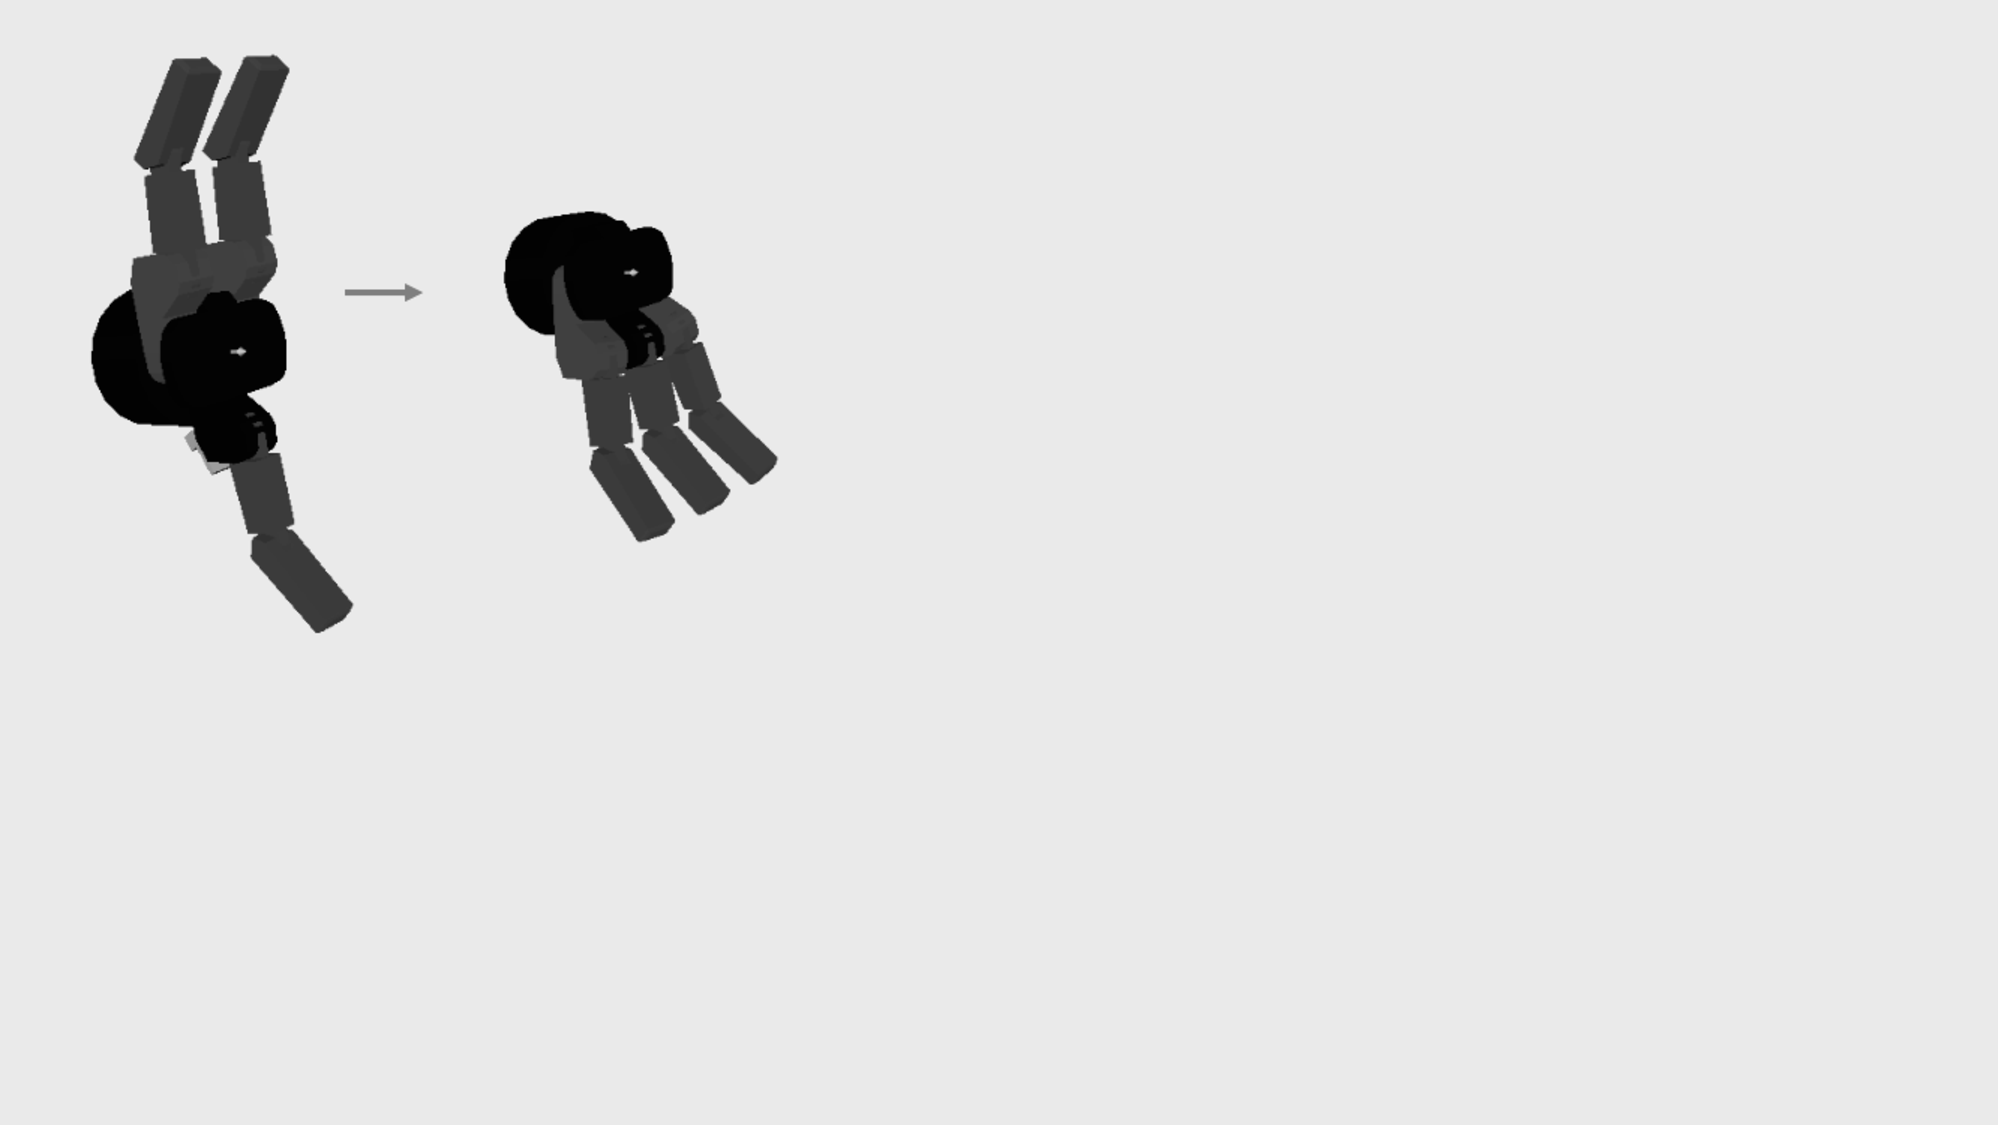
\includegraphics[trim={1cm 8cm 19cm 0cm},clip,width=1\linewidth,angle=0]{Apendices/Figuras/barret_eigengrasp_01.pdf}
				\caption{\textit{Eigengrasp} 01: fingers twist movement over wrist's normal axis.}
				\label{fig:barrett_eigengrasp01}
			\end{subfigure}
			\quad
			\begin{subfigure}[c]{.475\textwidth}
				\centering
				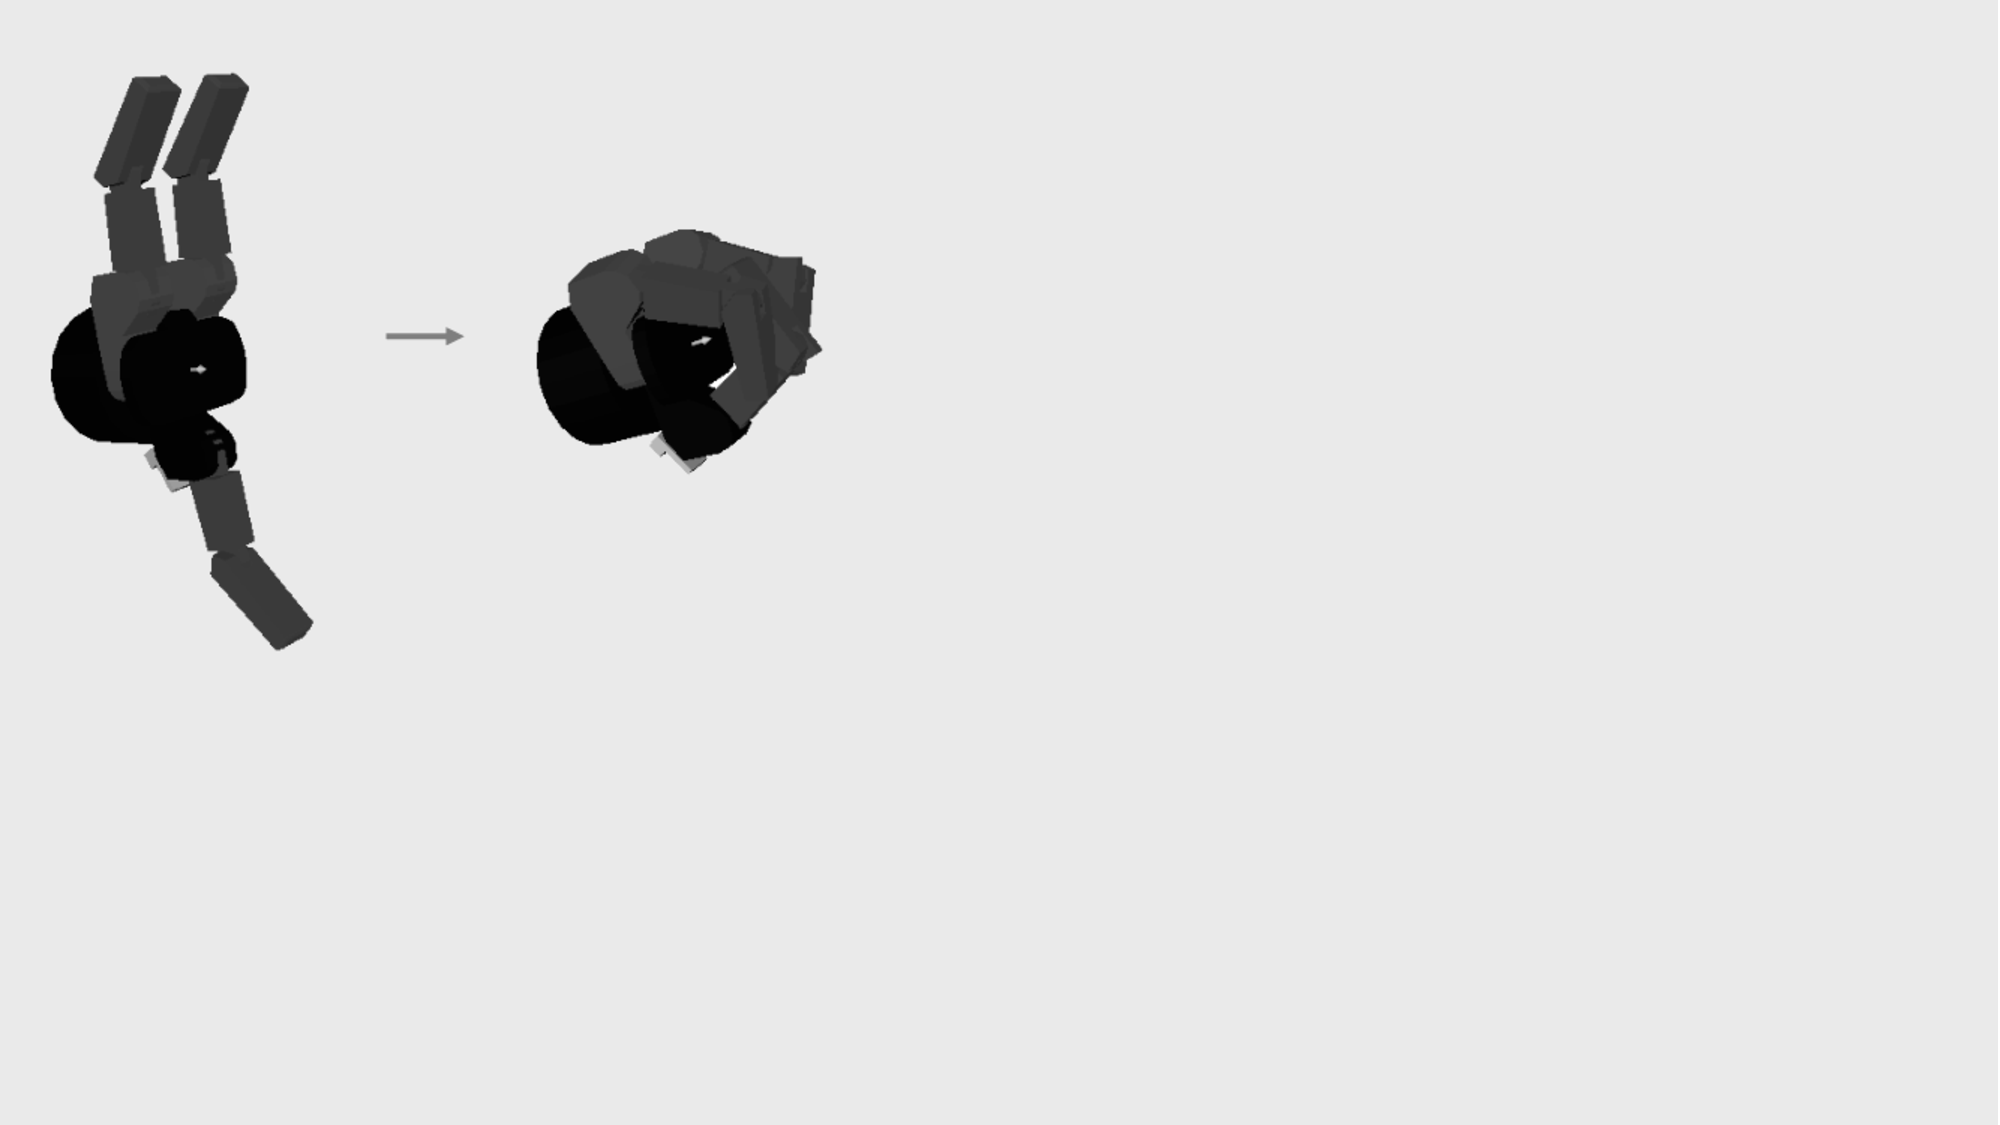
\includegraphics[trim={0.75cm 8cm 19cm 0.85cm},clip,width=1\linewidth,angle=0]{Apendices/Figuras/barret_eigengrasp_02.pdf}
				\caption{\textit{Eigengrasp} 02: fingers flexion.}
				\label{fig:barrett_eigengrasp02}
			\end{subfigure}
		\end{tcolorbox}
		\caption{The 4 \ac{DOF} Barrett gripper and its bidimensional \textit{eigengrasp} representation. }
		\label{fig:barrett_eigengrasps}
	}%end of resize box      
\end{figure}

The optimisation algorithm tries to minimize the distance from the \ac{ICP}, that constitute the \ac{ICR} (Figure~\ref{fig:icp_opt}), to the object surface by adjusting the discussed optimization variables $\mathbf{a}$ and $\mathbf{w}$. The \ac{ICR} is a contact region model (a predefined group of distributed \acp{ICP}) used to calculate the interaction of the algorithm, thus it is possible to create a feasible procedure. 

Therefore, the objective function to be minimised is describe by Equation~\ref{eq:fob_grasp_complete}, where $N$ is the number of total contacts in \ac{ICR}, $\mathbf{\hat{n}}_{i}$ is the surface normal, $\mathbf{o}_{i}$ the distance between the \ac{ICP} and the object ($i \in N$). The scalar $\alpha$ is a range adjustment factor between the distance and the normalised dot product of the second sum part. It is important to note that the $\mathbf{o}_{i}$ and $\mathbf{\hat{n}}_{i}$ are updated according to 3D simulation interaction in the ``GraspIt!''~\cite{AndrewT2004}. %A detailed description of the algorithm procedure is presented in \cite{Ciocarlie2009}.    

\begin{equation}
Q=\sum_{i=1}^{N}\left(1-\delta_{i}\right)\hspace{0.5cm}\textnormal{with}\hspace{0.5cm}\delta_{i}=\frac{\left|\mathbf{o}_{i}\right|}{\alpha}+\left(1-\frac{\mathbf{\hat{n}}_{i} \cdot\mathbf{o}_{i}}{\left|\mathbf{o}_{i}\right|}\right)
\label{eq:fob_grasp_complete}
\end{equation}


\begin{figure}[h!] %because of cas-sc
\resizebox{1\textwidth}{!}{%
\begin{tcolorbox}
% \centerline{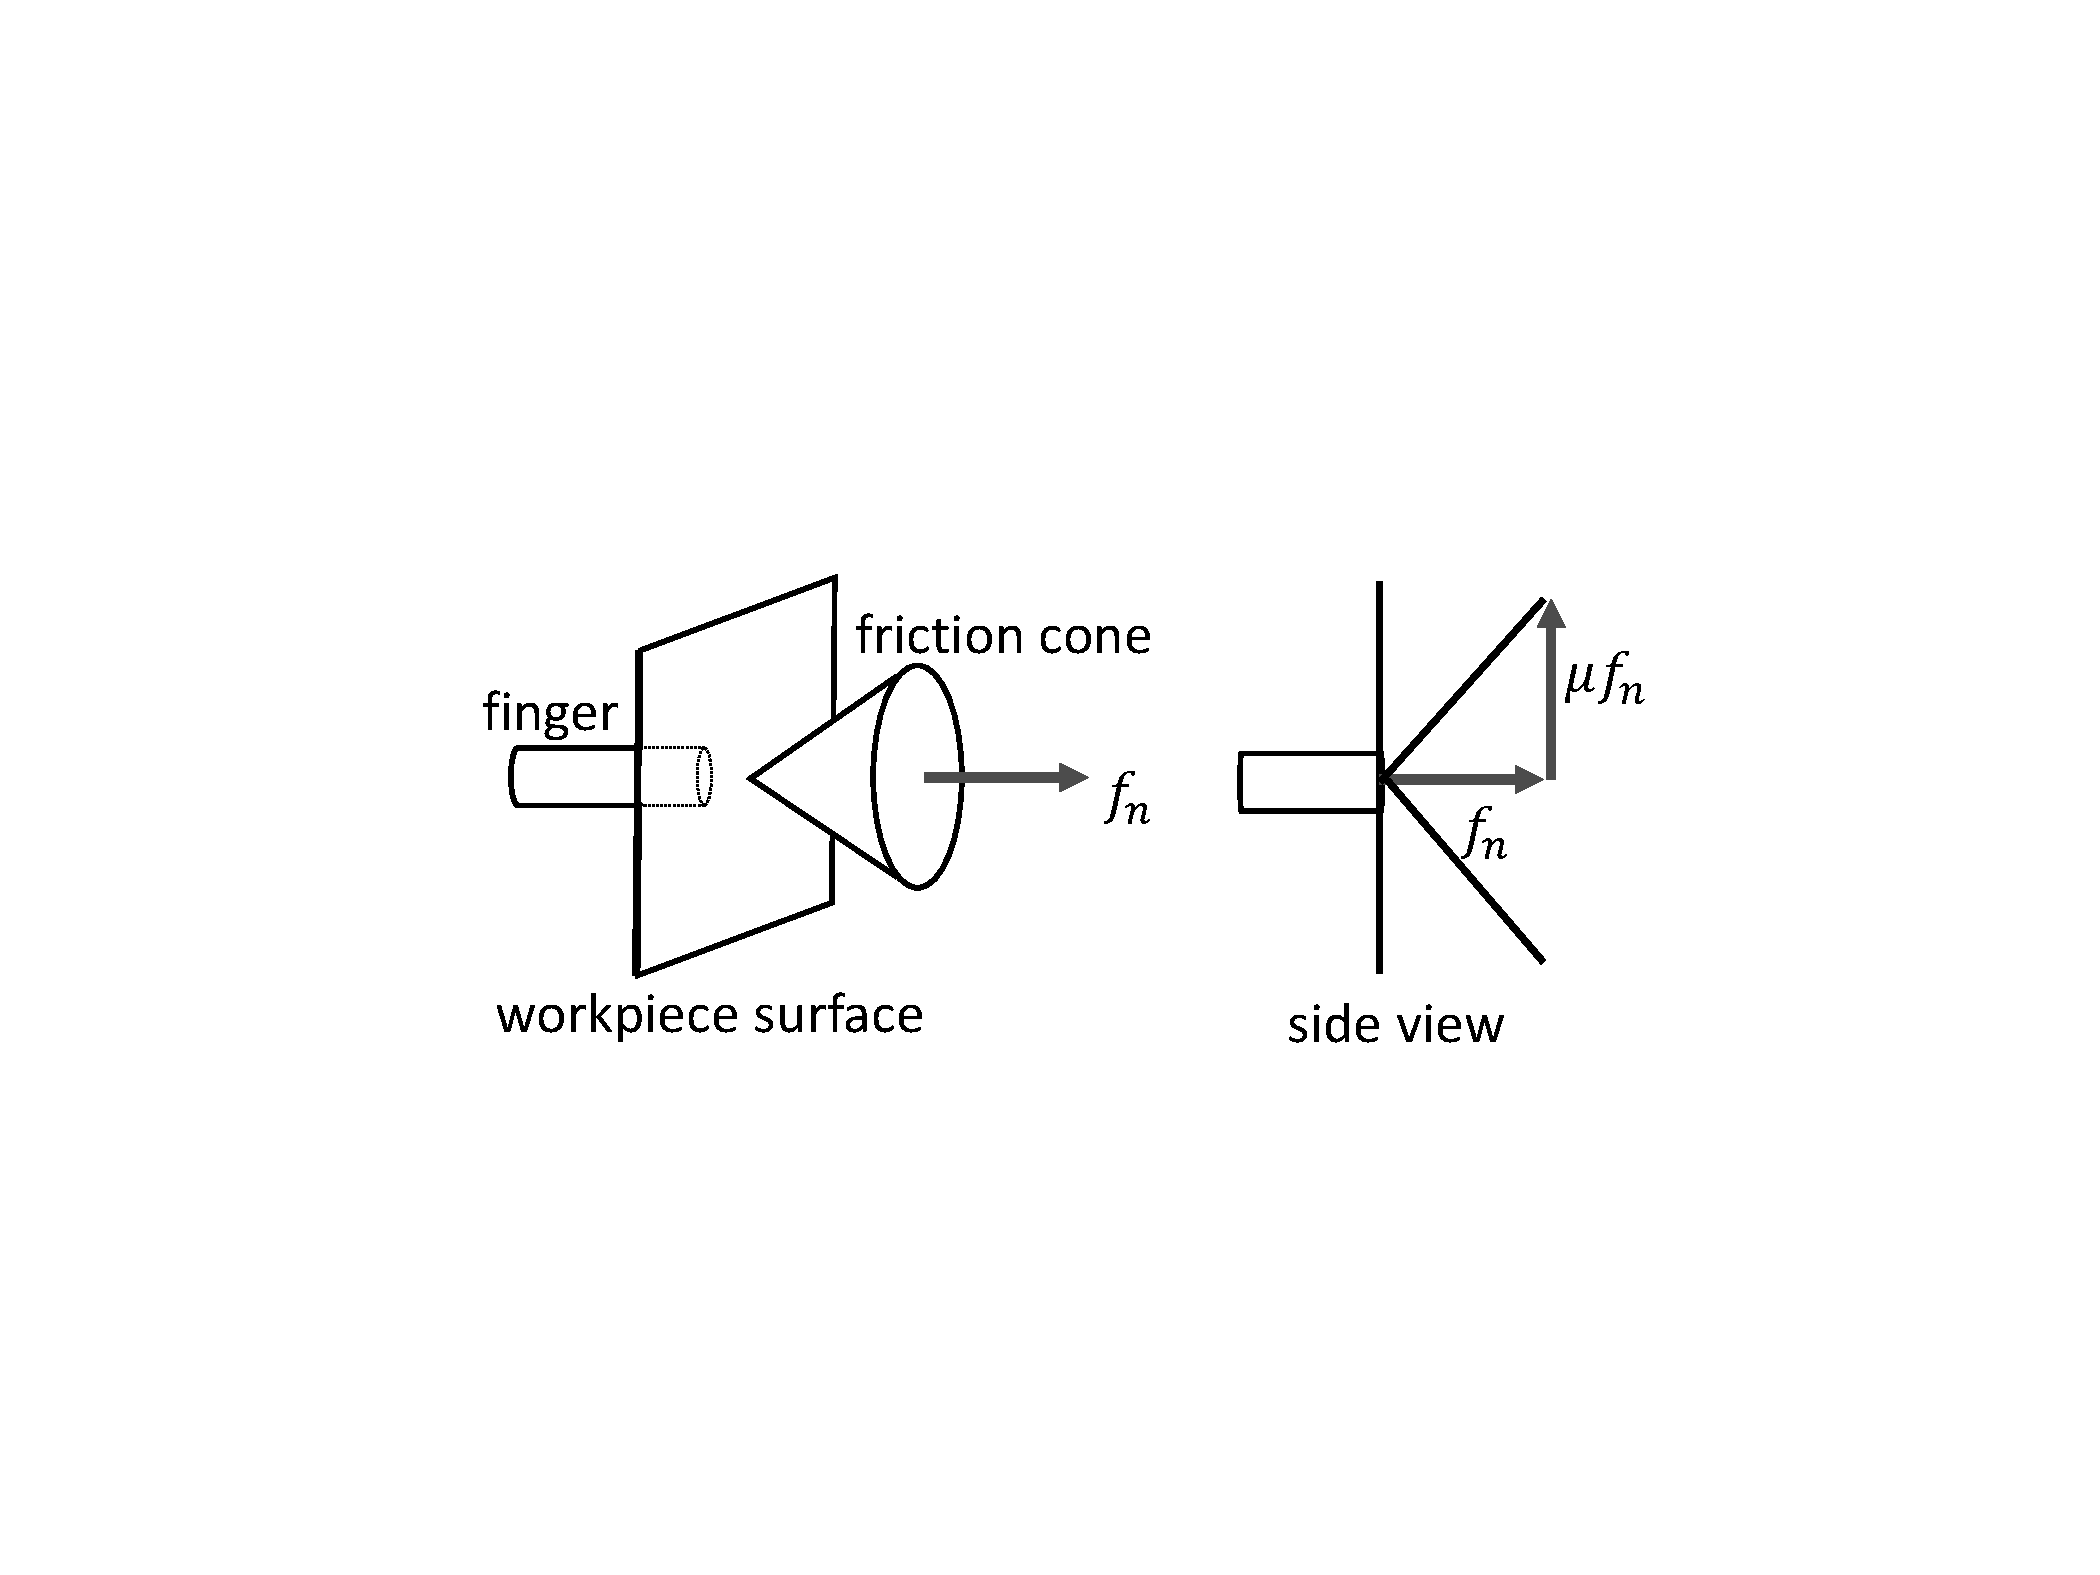
\includegraphics[trim={7cm 8cm 7cm 9cm},clip,width=1\linewidth,angle=0]{Cap2/Figuras/friction_contact.pdf}}
\centerline{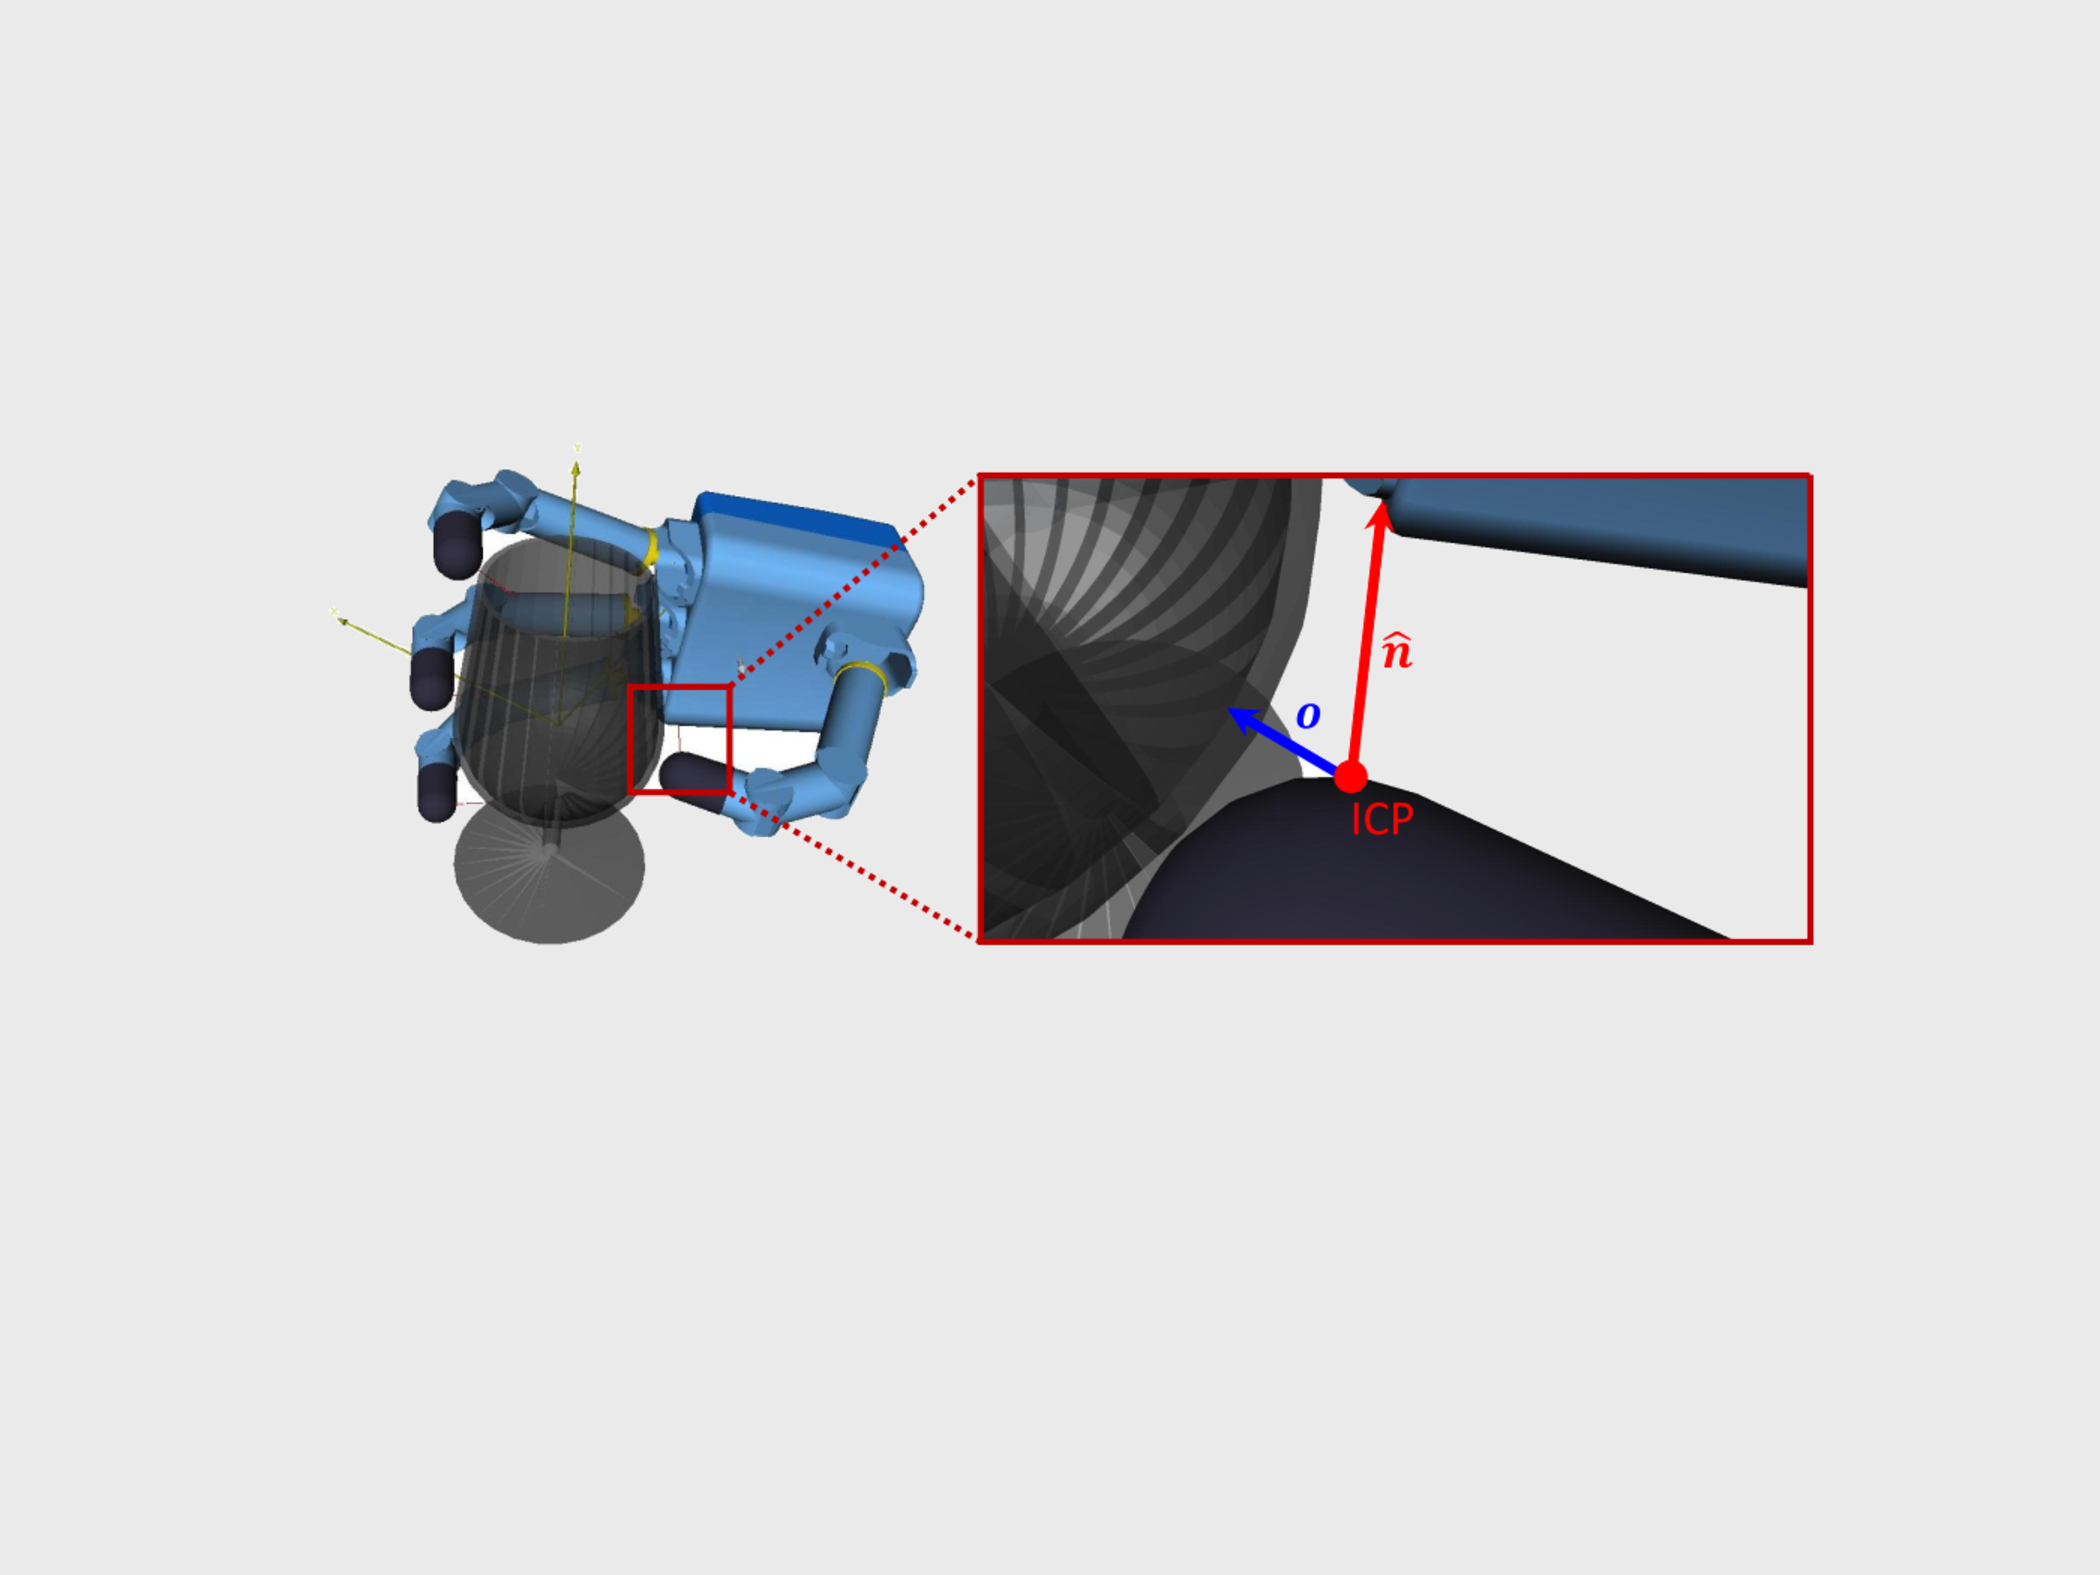
\includegraphics[trim={6.5cm 10cm 4cm 8cm},clip,width=1\linewidth,angle=0]{Apendices/Figuras/ICPreduction_gray_bg.pdf}}
\end{tcolorbox}
\caption{Grasping optimisation process elucidation.}
\label{fig:icp_opt}
}
\end{figure}


The algorithm proposed by~\cite{Ciocarlie2009}, and used in this proposal, is replicated in Algorithm~\ref{alg:snn_grasp}. As already mentioned, the variables that define the states are $\mathbf{a}$, related to the \textit{eigengrasp}, and $\mathbf{w}$, related to the wrist pose. The ``\textit{ObjFunc}'' is described by Equation~\ref{eq:fob_grasp_complete}. The ``\textit{Ngbr}'' is the calculus of the state variables neighbout valuer using the Equation~\ref{eq:neighbors} and, ``\textit{Probability}'' is the function to perform the jump probability to a new state according to Equation~\ref{eq:very_fast_snn_prob}. Since this step of the algorithm is based on ``GraspIt!''} the ``ForwardKinematics'' and collision check are are parts of this tool.

 \begin{algorithm}[h!]
 	\centering
	\resizebox{0.85\textwidth}{!}{%
	\begin{tcolorbox}
		\ForAll {variables of CurrentState} 
		{CurrentState.variable = RandomValue()}
		QCurrent = ObjFunc(CurrentState)\;
		Steps = 0\;
		QSaved = 0\;
		\While{Steps $\neq$ MaxSteps}{
			{Generate a new state as a neighbor of current state}\;
			\Repeat{legalState == true}
			{
				\ForAll{variables of NewState}{
					Sim. Annealing neighbor generation function\;
					NewState.variable = Ngbr(CurrentState.variable)\;
				}
				Apply ForwardKinematics(NewState)\;
				\If{collisions detected \textnormal{\textbf{or}} joint limits exceeded} {
					legalState = false\;
				} \Else{
					legalState = true
				}
				
			} 
			QNew = ObjFunc(NewState)\;
			\If{QNew $>$ QSaved}
			{
				Insert NewState in SavedStatesList\;
				QSaved = lowest ObjFunc value in SavedStateList\;
			}
			Sim. Annealing probability of "jumping" to new state\;
			PJump = Probability(QCurrent, QNew)\;
			\If{PJump $>$ 0.5}{
				CurrentState = NewState\;
				QCurrent = QNew\;
			}
			Steps = Steps + 1\;
		}	
		 \end{tcolorbox}
		\caption{\ac{SANN} applied to grasping}
		\label{alg:snn_grasp}
		}
\end{algorithm}
